\chapter{Results - Vicon Test}\label{cha4}
In this chapter the algorithm from chapter \ref{cha2} is tested under different conditions. In a first part (see chapter \ref{setup}) the set up of the test is presented. In the second part (see chapter \ref{evaluation}). The different test conditions are described and the results shown.
\section{Set up}\label{setup}
To verify the performance of the kalman filter algorithm described in chapter \ref{cha2} a ground truth is needed.  By using the motion capture system from the english company vicon some test were performed. The vicon system provides the position of the sensors and the orientation. Because this test has to be performed indoors no GPS signal was available. The vicon data for position added with some noise was simulated as GPS measurement of ekf and the derivative of the vicon's position added with some noise was pretended to be the velocity provided by the GPS. The impact of the noise can be seen in chapter \ref{noise}.
The pendulum was set as it can be seen on the picture in figure \ref{pend_setup}. 
\begin{figure}[h]
\centering
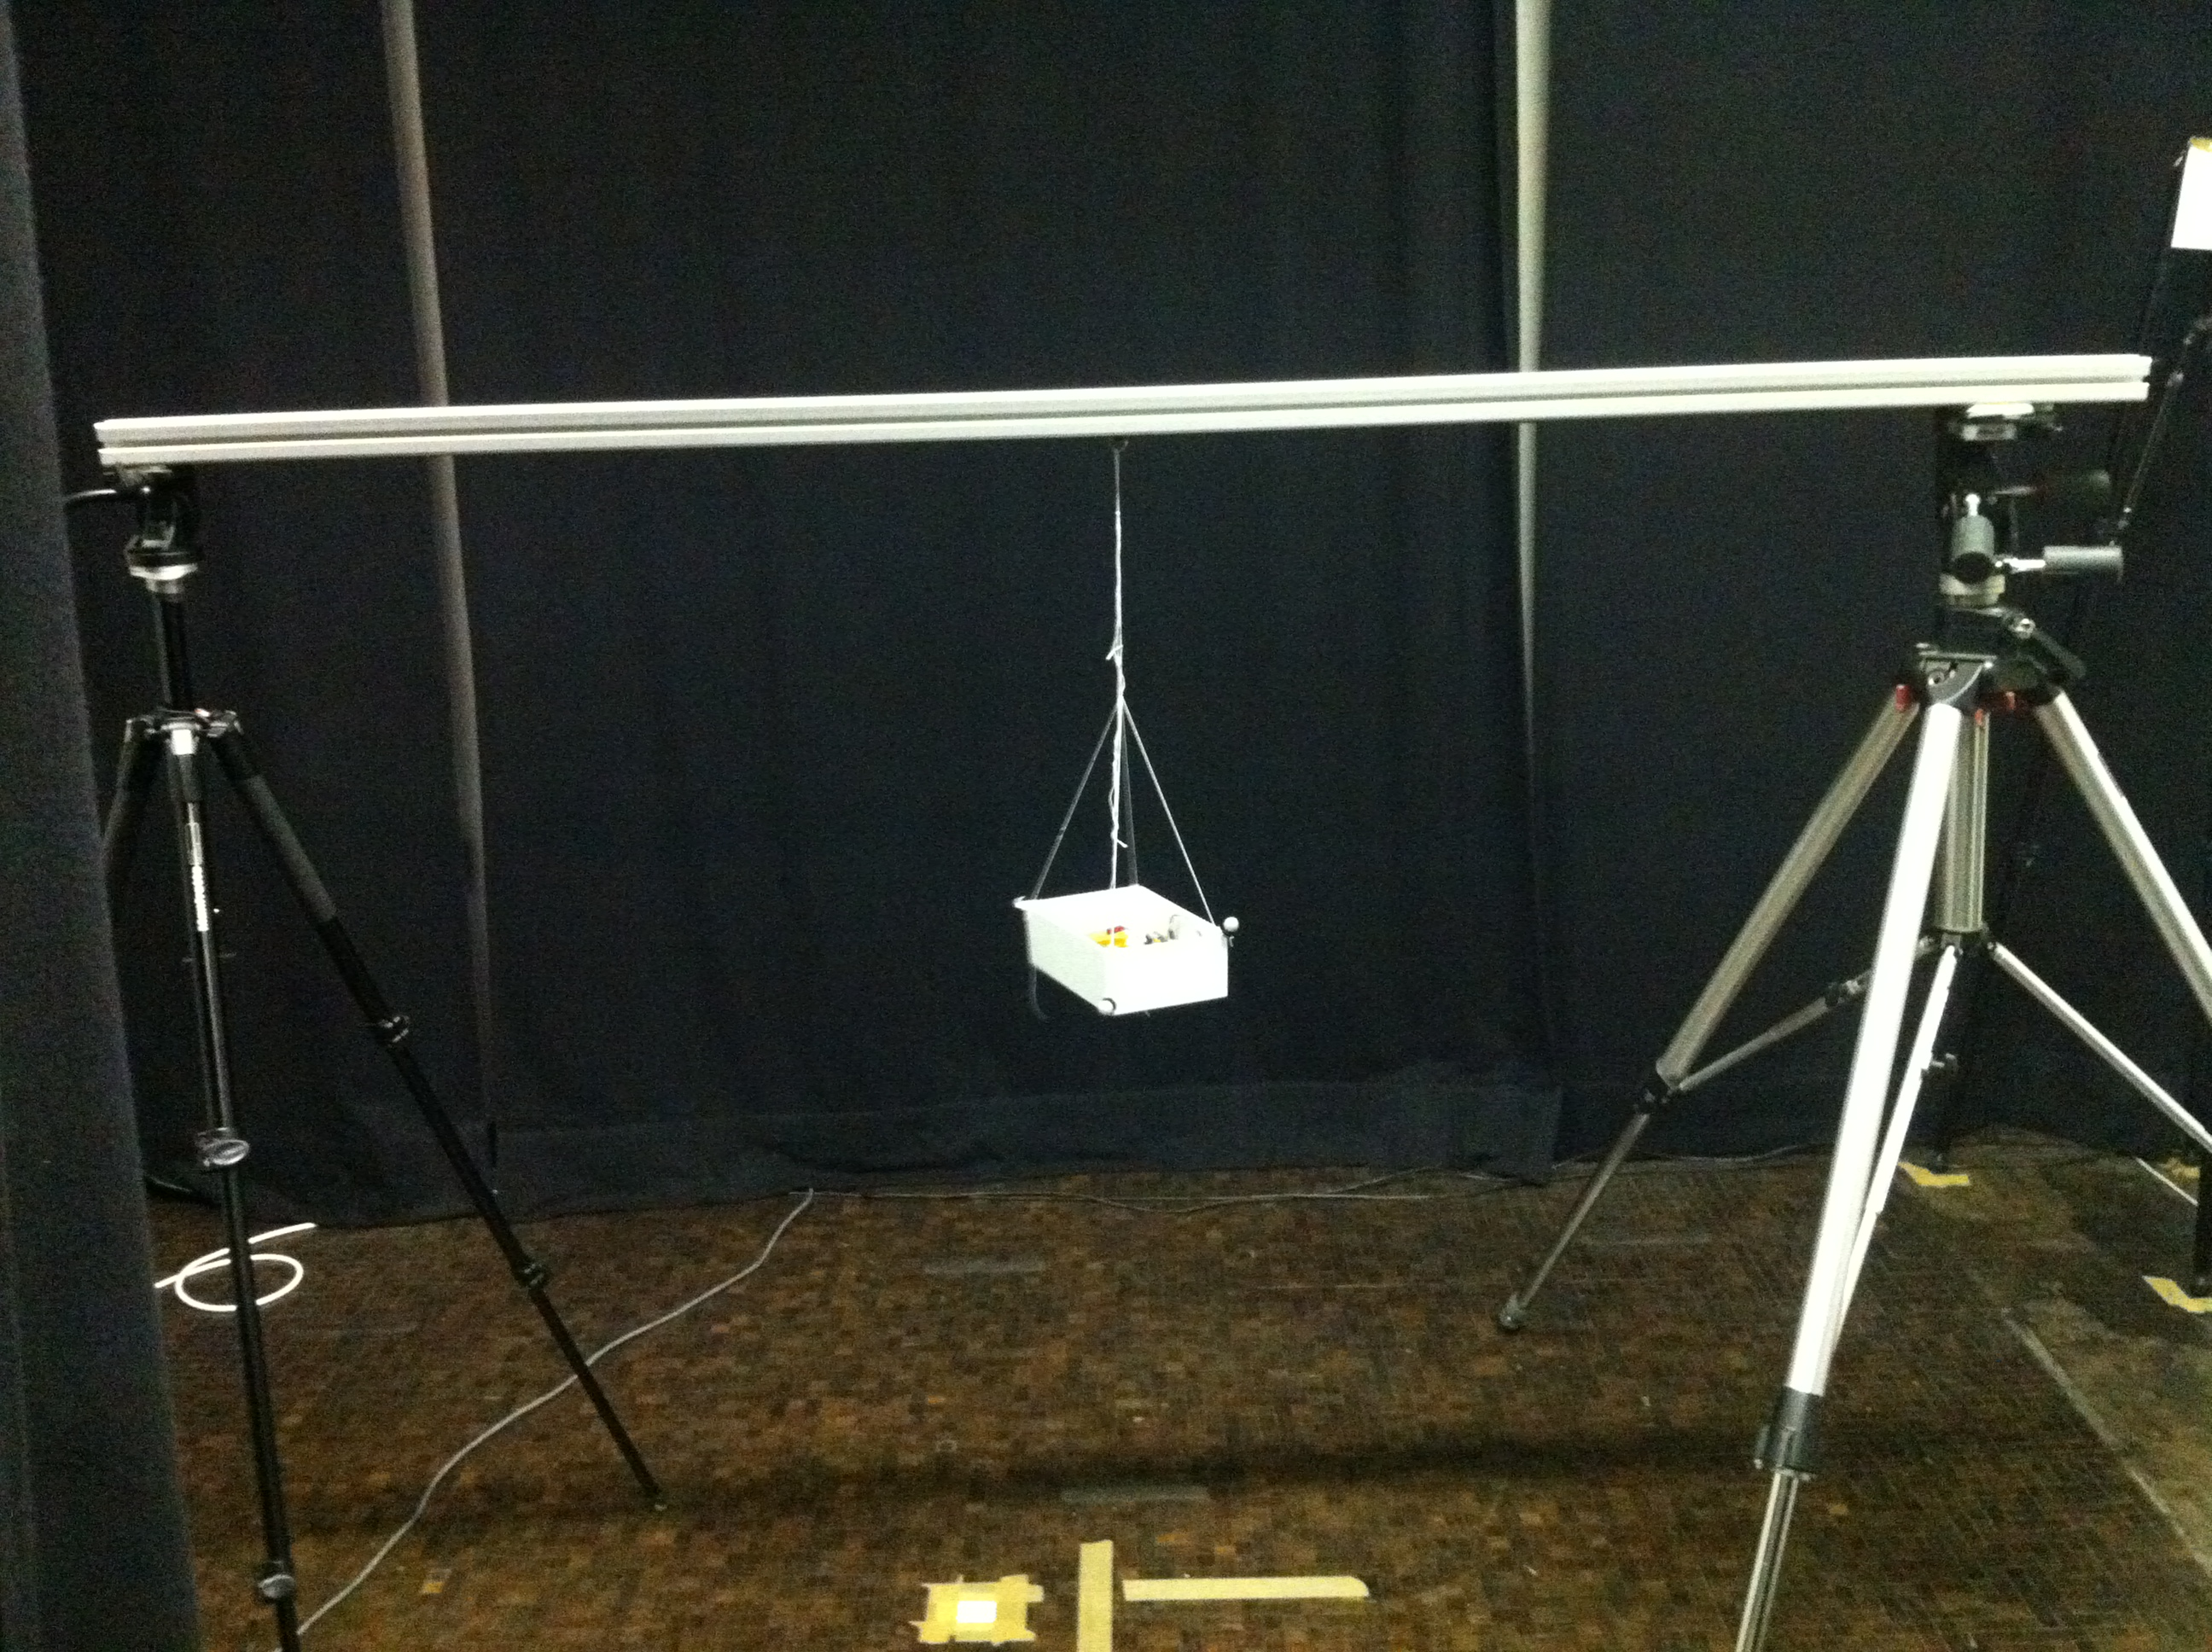
\includegraphics[width=0.8\textwidth]{vicon_bilder/IMG_0137.jpg}
\caption{Pendulum set up.}
\label{pend_setup}
\end{figure}
The box with the two sensors PX4 and MTi-G is showed in figure (...).
\begin{figure}[h]
\centering
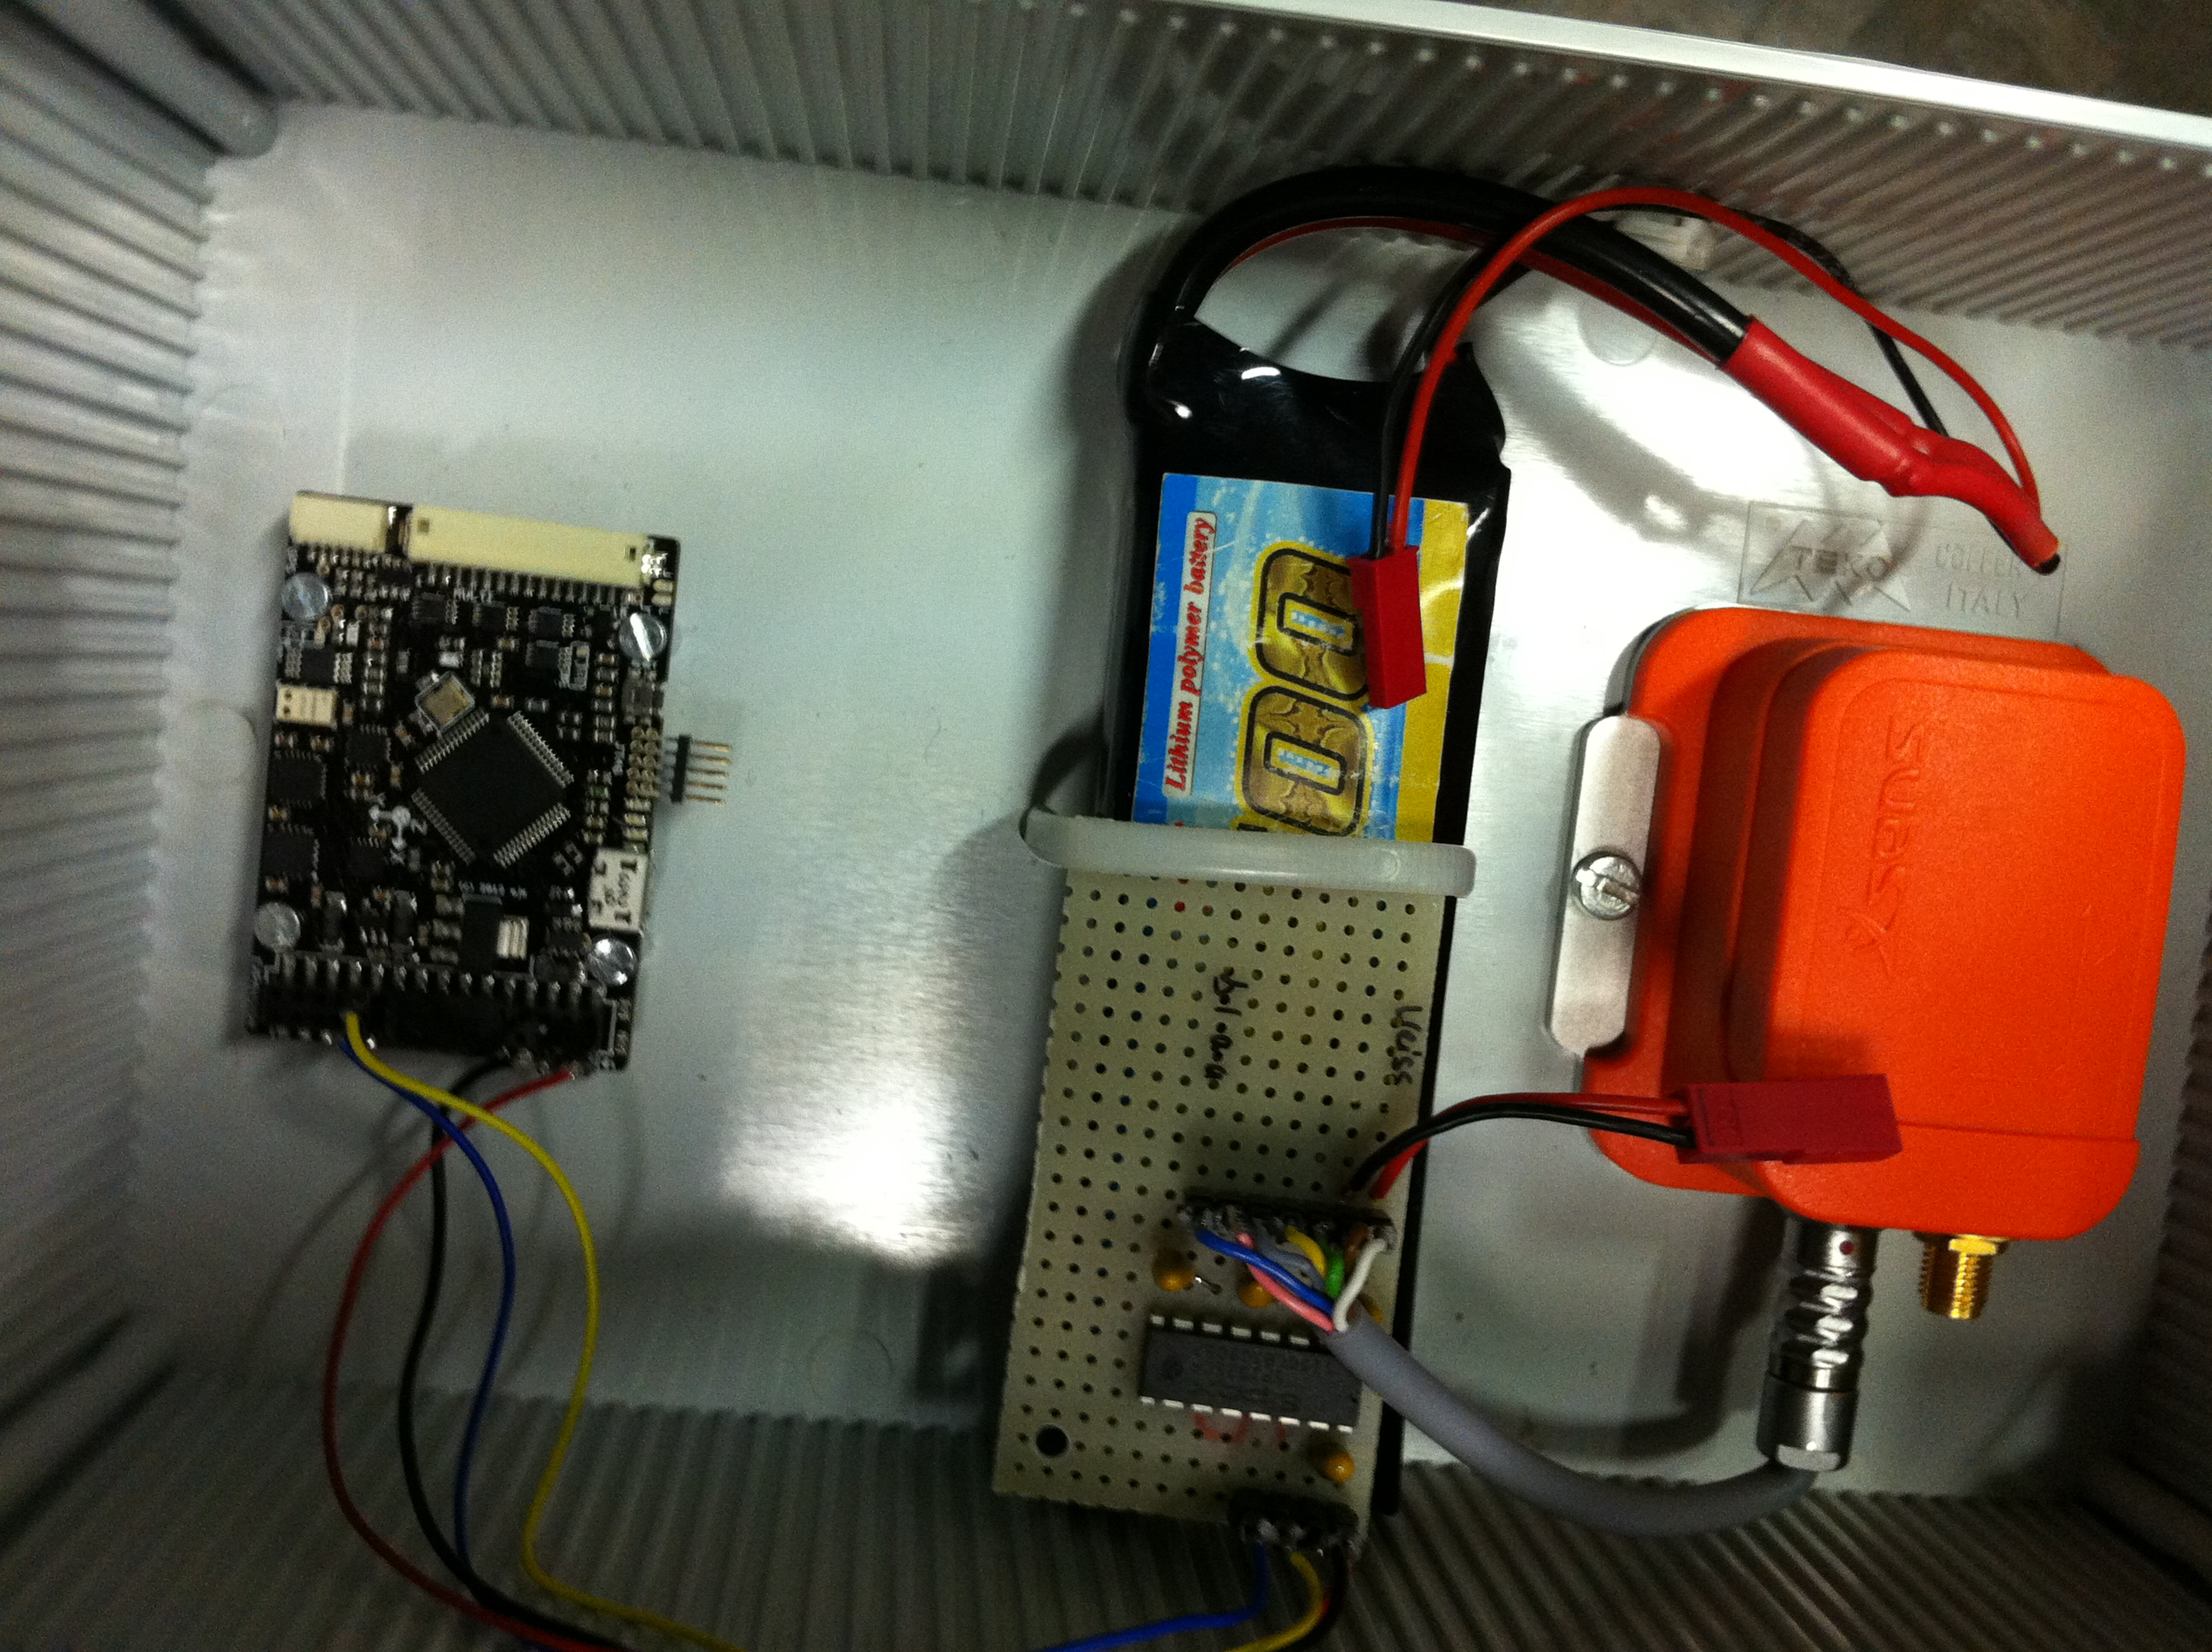
\includegraphics[width=0.8\textwidth]{vicon_bilder/IMG_0130.jpg}
\caption{Box with sensors.}
\label{box_setup}
\end{figure}
How the ekf state estimation differs depending weather the measurements are used from the PX4 IMU or from the Mti-G IMU can be read in chapter \ref{IMU_comp}.
In addition to that a kalman filter which does not take into account the information of a pendulum's movement has to be implemented. A free mass model state estimation is used as control algorithm. The varying results between the state estimation with using the pendulum's physical behavior and without are shown in chapter (..).
\section{Evaluation}\label{evaluation}
Four comparisons are made to get an overview of the estimators performance. This chapter shows how different test conditions influence the performance. In chapter \ref{noise} the estimator is tested once with a low noise GPS and one with a higher noise GPS signal. Since a GPS is not always received or has at least a lower frequency than the IMU measurements, the behavior of the estimator without GPS is a main performance criteria for an estimator. In chapter \ref{no_GPS} this condition is tested. How the measurements of different IMUs are influencing the estimator is shown in chapter \ref{IMU_comp}. Of course it has to be verified if an estimator using a the information of the pendulums physical behavior is more accurate than a estimator not using this information. The results of this question can be seen in chapter \ref{}. 
\subsection{Noise of the GPS}\label{noise}
The quality of the received GPS signal can vary according to different circumstances. The weather conditions or  an acceleration as we have seen in chapter \ref{cha2} can have an influence on the signals quality. As mentioned before is the GPS signal in the vicon test only simulated according the vicon data. This has the advantage of being able to use a GPS with different SNR since this is artificially added on the vicon's position data.
In figure \ref{detail_5snf} an SNR of 5 dB is added and in figure \ref{detail_25snr} a SNR of 25 dB is added.
\begin{figure}[h]
\centering
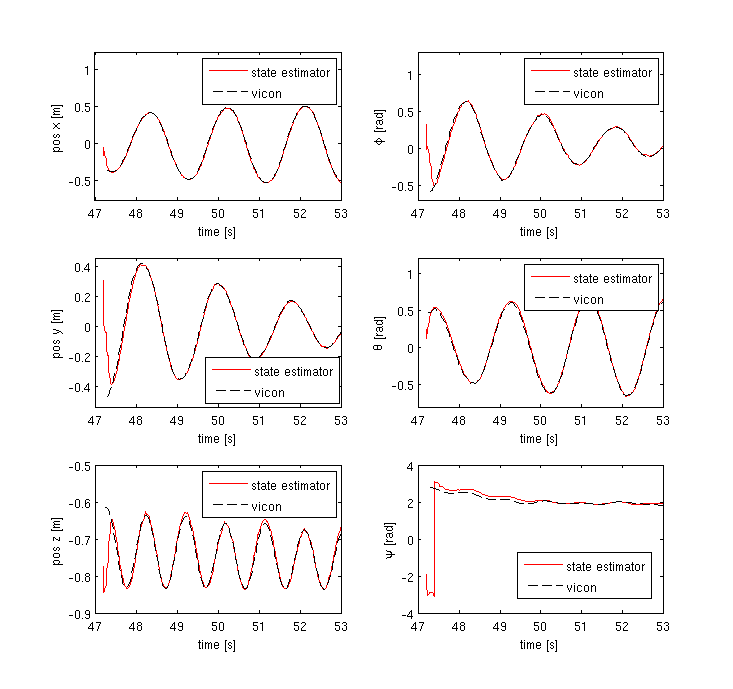
\includegraphics[width=1\textwidth]{pictures/2_2_SNR5_detail_GPS.png}
\caption{GPS signal with a SNR of 5 dB.}
\label{detail_5snr}
\end{figure}
\begin{figure}[h]
\centering
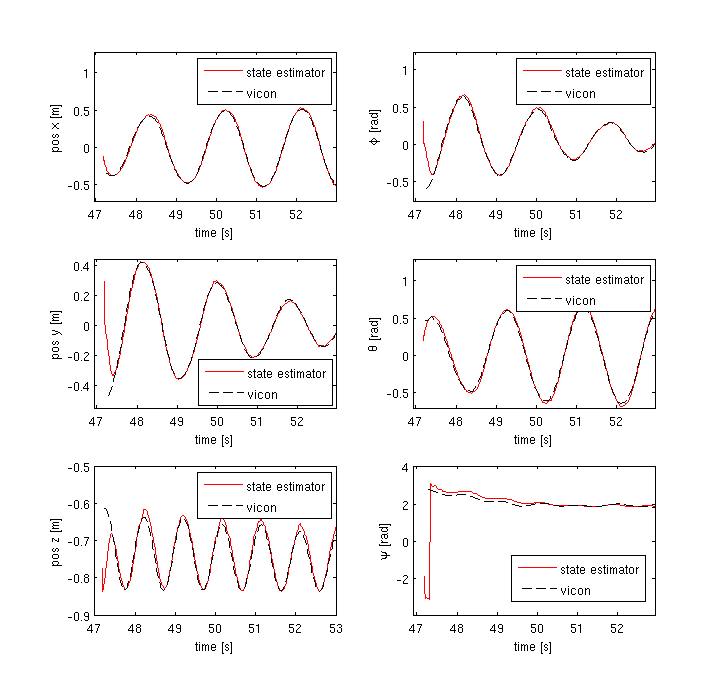
\includegraphics[width=1\textwidth]{pictures/2_2_SNR25_detail_GPS.png}
\caption{GPS signal with a SNR of 25 dB.}
\label{detail_25snr}
\end{figure}
The estimator somehow differs but, the noise level does not have a strong impact. In the estimator are the noise covariance matrixes adjust depending on which SNR the signal has. In the first case of a $5\; dB$ SNR the noise of the GPS position and velocity are defined as $0.001$ and $0.01$ respectively. In the second case when having a noise level of $25\; dB$ the noise in the estimator is increased to $0.01$ for the position and $0.05$ for the velocity.
In figure \ref{error_5snr} and figure \ref{error_25snr} the errors in position and orientation are plot for the $5\; dB$ and $25\; dB$ GPS signal respectively. 
\begin{figure}[h]
\centering
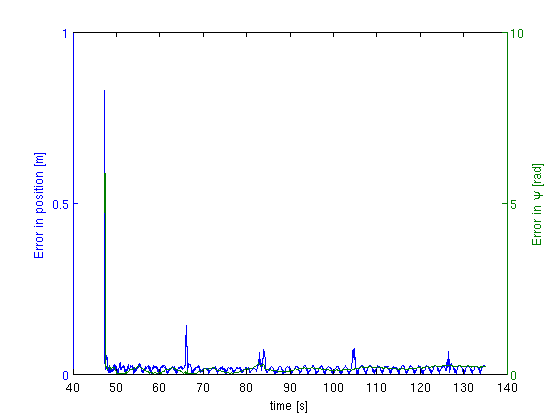
\includegraphics[width=1\textwidth]{pictures/2_2_SNR5_errors_GPS.png}
\caption{Error in position and orientation using a GPS signal with a SNR of 5 dB.}
\label{error_5snr}
\end{figure}
\begin{figure}[h]
\centering
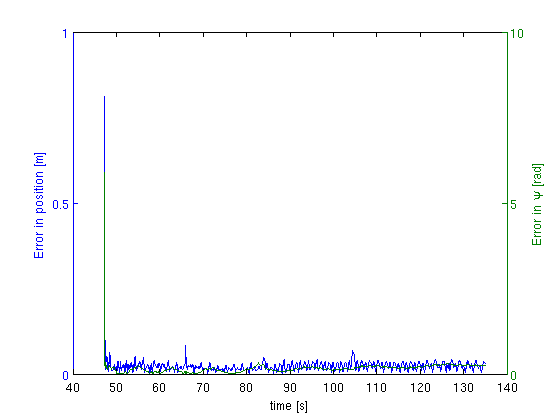
\includegraphics[width=1\textwidth]{pictures/2_2_SNR25_errors_GPS.png}
\caption{Error in position and orientation 	using a GPS signal with a SNR of 25 dB.}
\label{error_25snr}
\end{figure}
The error is calculated by the norm of the difference between estimated position and the effective position: 
\begin{equation}
error&=& \left\vert \begin{bmatrix} vicon_{pos\;x} \\ vicon_{pos\;y} \\ vicon_{pos\;z} \end{bmatrix}-\begin{bmatrix}state_{pos\;x} \\ state_{pos\;y} \\ state_{pos\;z} \end{bmatrix}
\end{equation}
For the orientation only the error of the first angle is calculated since the other two depend on the first one. When calculating the mean value of the error, starting at the point, when the GPS signal is settled down, following results are obtained:
\begin{eqnarray}
meanError_{pos}^{5\;dB}&=&0.0162\;m \\ meanError_{pos}^{25\;dB}&=&0.0223\;m \\ meanError_{\Theta}^{5\;dB}&=& 0.1440\;rad\\ meanError_{\Theta}^{25\;dB}&=& 0.1584 \;rad
\end{eqnarray}
And a ration of:
\begin{eqnarray}
\frac{meanError_{pos}^{5\;dB}}{meanError_{pos}^{25\;dB}}&=&0.7265 \\ \frac{meanError_{\Theta}^{5\;dB}}{meanError_{\Theta}^{25\;dB}}&0&0.9091
\end{eqnarray}
\subsection{GPS outage}\label{no_GPS}
Since explained before is the performance of a estimator without having a GPS signal an important criteria. In figure \ref{detail:_noGPS} a detail of the plot is shown.
\begin{figure}[h]
\centering
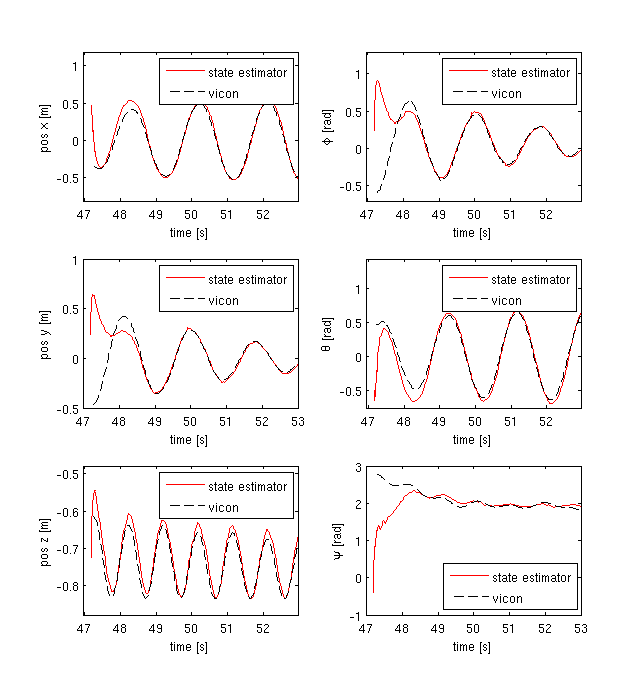
\includegraphics[width=1\textwidth]{pictures/2_2_detail_noGPS.png}
\caption{Estimation of the states without GPS signal.}
\label{detail_noGPS}
\end{figure}
The estimator is able to estimate the state only by using the IMU measurements. In this case the MTi-G data is used. Again can the error of the estimated position and the true position be calculated and plot as well as the difference between the estimated angle of $\Theta$ and the true angle as it is done in figure (..). The mean value of this error is calculated in the same way as the error between the different noise levels in chapter \ref{noise}: The ratios of error of the estimation with and without GPS are shown in equation:
\subsection{The MTi-G unit versus the PX4 unit}\label{IMU_comp}
In this section the influence of different measurements on the estimator are presented. The above test of the  estimator without having a GPS signal is carried out again with the PX4 measurements. In figure \ref{detail_no_GPS_P} the same detail is shown. 
\begin{figure}[h]
\centering
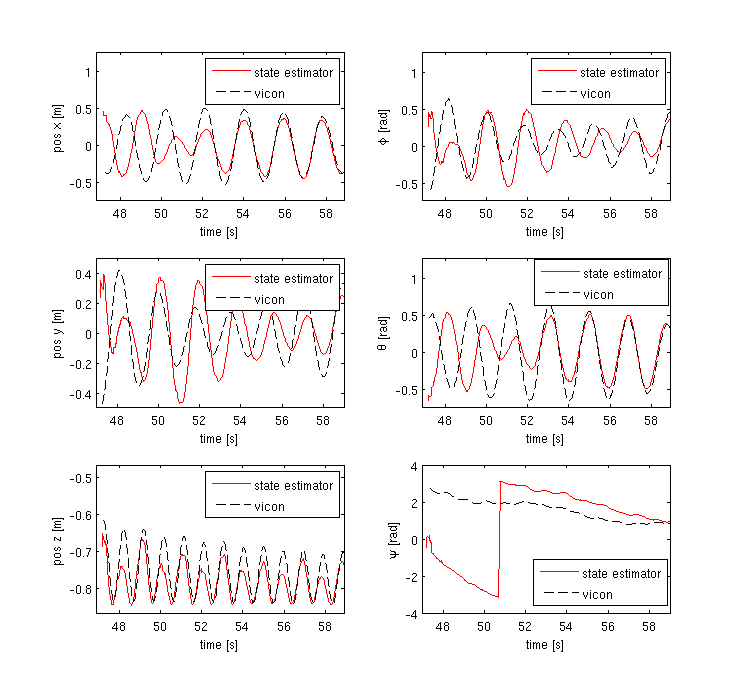
\includegraphics[width=1\textwidth]{pictures/2_2_P_detail_noGPS.png}
\caption{Estimation of the states without GPS and the help of the PX4 IMU.}
\label{detail_noGPS_P}
\end{figure}
The error is plot in figure \ref{error_noGPS_P}. 
\begin{figure}[h]
\centering
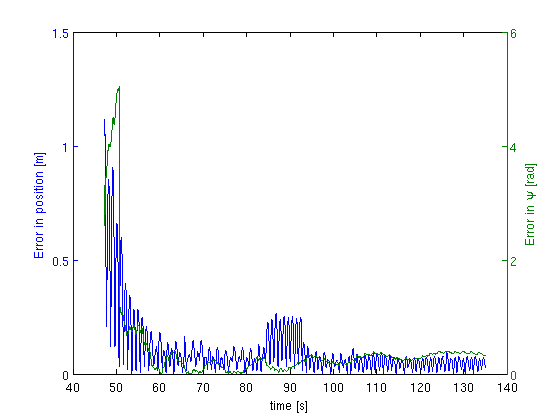
\includegraphics[width=1\textwidth]{pictures/2_2_P_errors_noGPS.png}
\caption{Error of the estimation of the states without GPS and the help of the PX4 IMU.}
\label{error_noGPS_P}
\end{figure}
The calculation of the ratios shows the big impact of the measurement unit.

\begin{table}[h]
\centering
\begin{tabular}{|c|c|c|c|c|}
 \hline
 Ratios &  meanError_{pos}^{5\;dB} & meanError_{pos}^{25\;dB} & meanError_{pos}^{no GPS\;MTi-G} & meanError_{pos}^{no GPS\;PX4} \\
 \hline
 meanError_{pos}^{5\;dB} & $ 1$ && &     \\
 \hline
 meanError_{pos}^{25\;dB} & & $1$ & &  \\
 \hline
 meanError_{pos}^{no GPS\;MTi-G} &  & & 1 &   \\
\hline
meanError_{pos}^{no GPS\;PX4} & & & & 1\\
\hline
\end {tabular}
\caption{ratio pos.}
\label{ratio_pos}
\end{table}



